\chapter{Studi Literatur}

\section{Pengantar Kriptografi}
Menurut \textcite{schneier1996}, Kriptografi merupakan ilmu pengetahuan dan seni yang berujuan untuk menjaga sebuah pesan tetap aman. Menurut \textcite{anderson2008}, Kriptografi dianggap sebagai pintu para pengembang keamanan untuk bertemu dengan ilmu matematika. Hal ini dapat terlihat bahwa banyak sekali algoritma kriptografi yang terkait dengan konsep matematika. Kriptografi dianggap juga sebagai seni. Menurut \textcite{munir2019}, hal ini dikarenakan dari pandangan sejarah berkembangnya kriptografi. Kriptografi ini terbentuk dikarenakan adanya keinginan untuk merahasiakan sebuah pesan. Tentu saja, setiap orang memiliki ciri khas serta caranya tersendiri untuk menyandikan sebuah pesan. Oleh karena itu, kriptografi dapat dianggap sebagai seni untuk merahasiakan sebuah pesan. 

Kriptografi pada dasarnya memiliki beberapa layanan dasar yang dapat digunakan dalam dunia keamanan. Menurut \textcite{schneier1996}, beberapa layanan yang terdapat pada kriptografi adalah sebagai berikut:
\begin{itemize}
  \item Kerahasiaan (\emph{confidentiality}) merupakan sebuah layanan yang diberikan oleh kriptografi untuk menjaga pesan agar pesan hanya dapat dimengerti oleh pihak yang memiliki otoritas. 
  \item Integritas (\emph{integrity}) merupakan layanan yang menjamin bahwa pesan yang diterima merupakan pesan yang belum pernah dilakukan modifikasi sebelumnya. Layanan ini menjamin data yang diterima sama dengan data tersebut saat pertama kali dikirim.
  \item Otentikasi (\emph{authentication}) merupakan layanan yang menjamin bahwa pesan yang diterima merupakan pesan yang dikirim oleh pengirim sesungguhnya. Hal ini terkait dengan klaim bahwa pesan yang dikirimkan tentu saja dapat dilakukan dekripsi dengan kunci yang telah disepakati.
  \item Anti penyangkalan (\emph{non-repudiation}) merupakan layanan yang menjamin bahwa pengirim tentu saja tidak akan dapat menyangkal pesan yang telah dia kirimkan.
\end{itemize} 

\section{Kriptografi Modern}
Kriptografi modern, menurut \textcite{munir2019}, merupakan kriptografi yang bekerja pada komputer digital. Pesan tidak hanya terbatas pada tulisan dan alfabet, namun pesan juga dapat berupa berbentuk apapun selama dapat diubah menjadi bentuk biner. Dalam Kriptografi modern, terdapat sebuah konsep yang disebut dengan kriptografi kunci publik, konsep fungsi \emph{hash}, serta tanda tangan digital. Hal ini merupakan konsep baru yang dapat digunakan untuk menjamin integritas serta anti penyangkalan dari pengirim pesan.

Menurut \textcite{schneier1996}, keamanan kriptografi modern tidak hanya cukup apabila merahasiakan algoritma penguncian. Hal ini dikarenakan apabila sebuah algoritma penguncian dapat dipecahkan, algoritma tersebut perlu diganti dengan yang baru. Dalam kriptografi modern, kerahasiaan yang perlu dijaga terletak pada kunci. Setiap operasi enkripsi serta dekripsi tentu saja akan melibatkan kunci ini. 

\subsection{Algoritma Kriptografi Modern}

Sebuah Algoritma modern tentu membutuhkan kunci untuk melakukan proses enkripsi dan dekripsi. Menurut \textcite{schneier1996}, algoritma kriptografi dapat dibagi menjadi dua, yaitu Kriptografi kunci simetrik dan kriptografi publik. Perbedaan dari kedua buah algoritma tersebut terletak pada kunci yang digunakan untuk melakukan enkripsi serta dekripsi pesan. 

Menurut \textcite{munir2019}, algoritma kunci simetri menggunakan kunci yang sama saat melakukan proses enkripsi serta dekripsi pesan. Asumsi yang diterapkan pada penggunaan algoritma ini adalah pengirim serta penerima sudah melakukan proses pembagian kunci. Skema proses enkripsi digambarkan pada gambar \ref{fig:crypto.symetric}. Beberapa contoh algoritma yang termasuk pada algoritma ini adalah \emph{Advanced Encryption Standard (AES)}, RC4, dan DES.

\begin{figure}[!h]
  \centering
  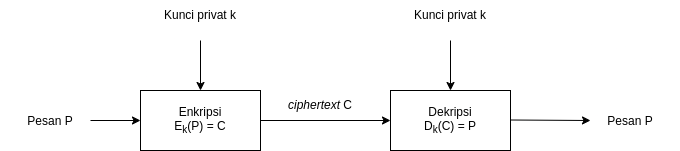
\includegraphics[width=\textwidth]{chapters/res/chapter-2/img/crypto.symetric.png}
  \caption{Visualisasi Proses Enkripsi Kriptografi Kunci Simetri} \label{fig:crypto.symetric}
  Sumber: \textcite{munir2019}
\end{figure}

Menurut \textcite{munir2019}, algoritma kunci publik (atau bisa disebut algoritma kunci nirsimetris) merupakan algoritma enkripsi yang menggunakan kunci yang berbeda pada saat melakukan proses enkripsi dan juga proses dekripsi. Pada saat melakukan komunikasi menggunakan algoritma ini, pihak yang terlibat harus memiliki satu buah kunci, yaitu kunci publik dan kunci privat. Pengirim pesan akan menggunakan kunci publik untuk mengunci pesan. Akan tetapi, penerima menggunakan kunci privat miliknya untuk membuka pesan. Dengan menggunakan algoritma ini, hanya penerima pesan yang dapat membuka pesan. Ilustrasi terkait enkripsi memanfaatkan algoritma ini terdapat pada Gambar \ref{fig:crypto.asymetric}. Beberapa contoh algoritma enkripsi kunci publik adalah RSA, \emph{Elgamal}, dan DSA.

\begin{figure}[!h]
  \centering
  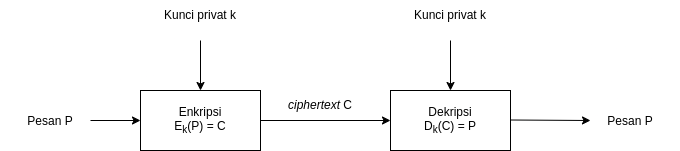
\includegraphics[width=\textwidth]{chapters/res/chapter-2/img/crypto.symetric.png}
  \caption{Visualisasi Proses Enkripsi Krpitografi Kunci Publik} 
  \label{fig:crypto.asymetric}
  Sumber: \textcite{munir2019}
\end{figure}

Menurut \textcite{munir2019}, keuntungan menggunakan kriptografi kunci publik ada dua. Keuntungan pertama adalah tidak adanya kebutuhan dalam mendistribusikan kunci rahasia. Kunci publik dapat dikirimkan melalui saluran yang tidak aman. Selain itu, keuntungan lain dari penggunaan kunci publik ini adalah jumlah pembuatan kunci dapat dikurangi. Pada saat menggunakan kriptografi kunci simetri, jumlah kunci yang harus dibuat adalah sebanyak jumlah pihak yang ingin berkomunikasi. Pada saat menggunakan algoritma asimetris, kunci yang perlu dibuat hanyalah sebanyak dua buah kunci, sehingga jumlah kunci menjadi lebih sedikit. 



\section{Pengantar Jaringan Komputer}
Testing 

\subsection{TCP Protocol}
Testing


\section{Pertukaran Kunci \emph{Diffie–Hellman}}
Testing 

\section{\emph{Advanced Encryption Standard (AES)}}
Testing

\section{Teori Chaos}
Testing

\section{Pembangkit Bilangan Acak yang Aman untuk Kriptografi}
Testing

\subsection{CSRPNG berbasis Chaos}
Testing

\section{Fungsi Hash Satu Arah}
Testing

\subsection{\emph{Secure Hash Algorithm (SHA)}}
Testing

\section{Penelitian Terkait}
Testing

\subsection{Sinkronisasi Kunci Dinamis berbasis Chaos den Aplikasinya pada Pengenkripsian Gambar dengan Algoritma AES yang diimprovisasi}
Testing

\subsection{Enkripsi Gambar dan Analisisnya memanfaatkan Algoritma AES dinamis}
Testing

\subsection{Peningkatan Keamanan Enkripsi AES menggunakan Algoritma \emph{Salt} Dinamis}
Testing
